% Options for packages loaded elsewhere
\PassOptionsToPackage{unicode}{hyperref}
\PassOptionsToPackage{hyphens}{url}
\PassOptionsToPackage{dvipsnames,svgnames,x11names}{xcolor}
%
\documentclass[
  letterpaper,
  DIV=11,
  numbers=noendperiod]{scrartcl}

\usepackage{amsmath,amssymb}
\usepackage{iftex}
\ifPDFTeX
  \usepackage[T1]{fontenc}
  \usepackage[utf8]{inputenc}
  \usepackage{textcomp} % provide euro and other symbols
\else % if luatex or xetex
  \usepackage{unicode-math}
  \defaultfontfeatures{Scale=MatchLowercase}
  \defaultfontfeatures[\rmfamily]{Ligatures=TeX,Scale=1}
\fi
\usepackage{lmodern}
\ifPDFTeX\else  
    % xetex/luatex font selection
\fi
% Use upquote if available, for straight quotes in verbatim environments
\IfFileExists{upquote.sty}{\usepackage{upquote}}{}
\IfFileExists{microtype.sty}{% use microtype if available
  \usepackage[]{microtype}
  \UseMicrotypeSet[protrusion]{basicmath} % disable protrusion for tt fonts
}{}
\makeatletter
\@ifundefined{KOMAClassName}{% if non-KOMA class
  \IfFileExists{parskip.sty}{%
    \usepackage{parskip}
  }{% else
    \setlength{\parindent}{0pt}
    \setlength{\parskip}{6pt plus 2pt minus 1pt}}
}{% if KOMA class
  \KOMAoptions{parskip=half}}
\makeatother
\usepackage{xcolor}
\setlength{\emergencystretch}{3em} % prevent overfull lines
\setcounter{secnumdepth}{5}
% Make \paragraph and \subparagraph free-standing
\ifx\paragraph\undefined\else
  \let\oldparagraph\paragraph
  \renewcommand{\paragraph}[1]{\oldparagraph{#1}\mbox{}}
\fi
\ifx\subparagraph\undefined\else
  \let\oldsubparagraph\subparagraph
  \renewcommand{\subparagraph}[1]{\oldsubparagraph{#1}\mbox{}}
\fi


\providecommand{\tightlist}{%
  \setlength{\itemsep}{0pt}\setlength{\parskip}{0pt}}\usepackage{longtable,booktabs,array}
\usepackage{calc} % for calculating minipage widths
% Correct order of tables after \paragraph or \subparagraph
\usepackage{etoolbox}
\makeatletter
\patchcmd\longtable{\par}{\if@noskipsec\mbox{}\fi\par}{}{}
\makeatother
% Allow footnotes in longtable head/foot
\IfFileExists{footnotehyper.sty}{\usepackage{footnotehyper}}{\usepackage{footnote}}
\makesavenoteenv{longtable}
\usepackage{graphicx}
\makeatletter
\def\maxwidth{\ifdim\Gin@nat@width>\linewidth\linewidth\else\Gin@nat@width\fi}
\def\maxheight{\ifdim\Gin@nat@height>\textheight\textheight\else\Gin@nat@height\fi}
\makeatother
% Scale images if necessary, so that they will not overflow the page
% margins by default, and it is still possible to overwrite the defaults
% using explicit options in \includegraphics[width, height, ...]{}
\setkeys{Gin}{width=\maxwidth,height=\maxheight,keepaspectratio}
% Set default figure placement to htbp
\makeatletter
\def\fps@figure{htbp}
\makeatother

\usepackage{booktabs}
\usepackage{longtable}
\usepackage{array}
\usepackage{multirow}
\usepackage{wrapfig}
\usepackage{float}
\usepackage{colortbl}
\usepackage{pdflscape}
\usepackage{tabu}
\usepackage{threeparttable}
\usepackage{threeparttablex}
\usepackage[normalem]{ulem}
\usepackage{makecell}
\usepackage{xcolor}
\KOMAoption{captions}{tableheading}
\usepackage{amsmath}
\usepackage{amssymb}
\usepackage{pgfplots}
\makeatletter
\@ifpackageloaded{caption}{}{\usepackage{caption}}
\AtBeginDocument{%
\ifdefined\contentsname
  \renewcommand*\contentsname{Table of contents}
\else
  \newcommand\contentsname{Table of contents}
\fi
\ifdefined\listfigurename
  \renewcommand*\listfigurename{List of Figures}
\else
  \newcommand\listfigurename{List of Figures}
\fi
\ifdefined\listtablename
  \renewcommand*\listtablename{List of Tables}
\else
  \newcommand\listtablename{List of Tables}
\fi
\ifdefined\figurename
  \renewcommand*\figurename{Figure}
\else
  \newcommand\figurename{Figure}
\fi
\ifdefined\tablename
  \renewcommand*\tablename{Table}
\else
  \newcommand\tablename{Table}
\fi
}
\@ifpackageloaded{float}{}{\usepackage{float}}
\floatstyle{ruled}
\@ifundefined{c@chapter}{\newfloat{codelisting}{h}{lop}}{\newfloat{codelisting}{h}{lop}[chapter]}
\floatname{codelisting}{Listing}
\newcommand*\listoflistings{\listof{codelisting}{List of Listings}}
\makeatother
\makeatletter
\makeatother
\makeatletter
\@ifpackageloaded{caption}{}{\usepackage{caption}}
\@ifpackageloaded{subcaption}{}{\usepackage{subcaption}}
\makeatother
\ifLuaTeX
  \usepackage{selnolig}  % disable illegal ligatures
\fi
\usepackage{bookmark}

\IfFileExists{xurl.sty}{\usepackage{xurl}}{} % add URL line breaks if available
\urlstyle{same} % disable monospaced font for URLs
\hypersetup{
  pdftitle={Various Demographic Factors Effect on Students' Participation In Extracurricular Activities},
  pdfauthor={Vanshika Vanshika; Navya Hooda; Shea Munson; Alexia Mbagaya; Chloe Syriac},
  colorlinks=true,
  linkcolor={blue},
  filecolor={Maroon},
  citecolor={Blue},
  urlcolor={Blue},
  pdfcreator={LaTeX via pandoc}}

\title{Various Demographic Factors Effect on Students' Participation In
Extracurricular Activities\thanks{Code and data are available at:
https://github.com/vanshikav2/Extra\_Curricular\_Activities\_Research/}}
\usepackage{etoolbox}
\makeatletter
\providecommand{\subtitle}[1]{% add subtitle to \maketitle
  \apptocmd{\@title}{\par {\large #1 \par}}{}{}
}
\makeatother
\subtitle{Data Collected from STA304H5F in 2024}
\author{Vanshika Vanshika \and Navya Hooda \and Shea Munson \and Alexia
Mbagaya \and Chloe Syriac}
\date{November 28, 2024}

\begin{document}
\maketitle
\begin{abstract}
It is known that for students to have a well-rounded university
experience, participation in extracurricular activities is vital, not
only for academic but personal growth. However, student participation in
extracurricular activities depends on a number of factors. Some include
scheduling and time-commitment factors, commute factors and the
diversity of student activities/clubs. This study aims to explore this
by investigating the reasons that students select certain
extracurricular activities at the University of Toronto Mississauga
(UTM) campus. An anonymous online survey on Google Forms was created for
students in a third-year Statistics course to complete. Findings showed
that there was no significant relationship between campus distance and
program of study with extracurricular involvement. Although there was
some gender influence on the participation of extra-curricular activity,
this variation is not statistically relevant as the p-value was 1. On
the other hand, there was a statistically significant monotonic
relationship (rho = 0.937) between time commitment and activity count.
As students increase their time commitment, so does their participation
in ECAs. Although results produced minimal significant findings, we
believe that this is a valiant step in the right direction towards
investigating student participation at UTM.
\end{abstract}

\renewcommand*\contentsname{Table of contents}
{
\hypersetup{linkcolor=}
\setcounter{tocdepth}{3}
\tableofcontents
}
\section{Introduction}\label{introduction}

An important part of having a healthy life in university is maintaining
a balance between school, work, and social life. Among other aspects, a
major part of many university students' social lives is extracurricular
activities (ECAs). Being such a major part of students' social lives,
determining what factors can negatively impact student participation in
ECAs is a critical step in helping minimize negative impacts on
students' wellbeing. In our study, we focused on students in STA304
students in Fall of 2024 and examined their levels of participation in
various kinds of ECA's. In particular, we analyzed if various
demographic factors affected students' participation in ECAs. As UTM is
primarily a commuter campus, of special interest was students living
distance from campus. To conduct our study, during the first three weeks
of October 2024 we distributed a survey on the STA304 Piazza Discussion
board to collect data on student demographics factors and information
relating to individual participation in ECAs. Our study consisted of
three research questions.

\subsection{Research Questions and
Hypotheses}\label{research-questions-and-hypotheses}

\begin{enumerate}
\def\labelenumi{\arabic{enumi}.}
\tightlist
\item
  \textbf{Research Question 1}: What is the most preferred type of
  extracurricular activity, and do demographic factors influence student
  preferences for certain extracurricular activities?

  \begin{itemize}
  \tightlist
  \item
    \(H_{0}\): Student demographic factors have no effect on
    participation in extracurricular activities.
  \item
    \(H_{a}\): Participation in extracurricular activities is affected
    by demographic factors.
  \end{itemize}
\item
  \textbf{Research Question 2}: Does proximity to campus affect
  participation in extracurricular activities?

  \begin{itemize}
  \tightlist
  \item
    \(H_{0}\): Proximity to campus has no effect on participation in
    extracurricular activities.
  \item
    \(H_{a}\): Students living further from campus will have lower
    participation rates.
  \end{itemize}
\item
  \textbf{Research Question 3}: Does timing/scheduling of
  extracurricular activities impact student participation in
  extracurricular activities?

  \begin{itemize}
  \tightlist
  \item
    \(H_{0}\): Timing/scheduling of extracurricular activities has no
    impact on student participation.
  \item
    \(H_{a}\): Participation in extracurricular activities is affected
    by their timing/scheduling.
  \end{itemize}
\end{enumerate}

\section{Data}\label{sec-data}

\subsection{Methodology}\label{methodology}

Data collection began in the first three weeks of October 2024, an
online anonymous survey on Google Forms was created for participants to
complete. This survey was created in order to investigate the reasons
that students select and participate in certain ECAs. This online survey
was posted to a Piazza thread where students can easily locate the
survey link. Although using Stratified Random Sampling where the strata
were the STA304 lecture sections (ie. LEC0101 and LEC0102) was proposed,
the sampling method that was truly used was Simple random sampling.
Nevertheless, randomness was ensured as the link to the survey was
posted to Piazza where everyone had the equal opportunity to complete
the survey and be chosen for the study. We collected a sample of 63
students. The survey consisted of 10 questions asking for details on
their lecture section, demographic information, program of study, and
distance from the UTM campus. We also included questions on the number,
types of activities and the time commitment of the ECAs they are
involved in. To encourage students to complete our online survey, we
asked participants to share a link to their group's survey, which we
would complete in return.

For computing the sample size from population size of \(N = 200\), we
chose a bound of \(B = 0.1047\) and calculated with an approximation of
\(p = 0.5\). Calculating a sample size using
\(n = \frac{Npq}{(N-1)\frac{B^2}{4}+pq}\) gives
\(\frac{200*0.25*0.25}{(200-1)*\frac{0.1047^2}{4}+0.25} = 62.8643 \approx 63\)

\section{Analysis}\label{sec-data1}

The majority of the analysis for our research questions is based on the
various student demographic factors. As such, it is worthwhile to go
over, in a preliminary fashion, the results of our survey to give
further background on the study before continuing into the analysis of
the research questions.

We had a slightly higher response rate from students in LEC0101,
approximately a 6:4 ratio.

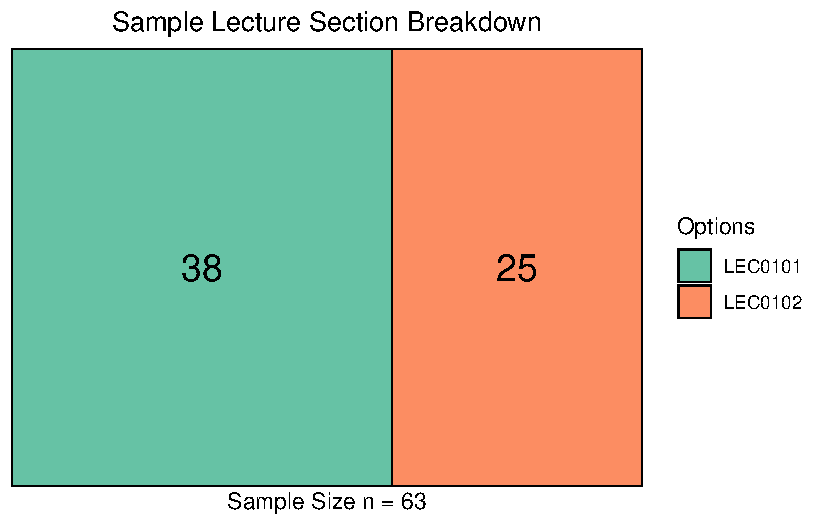
\includegraphics{technical_report_files/figure-pdf/p1-1.pdf}

Our sample indicated a higher percentage of males vs females, with no
students responding with Other or Prefer Not to Answer

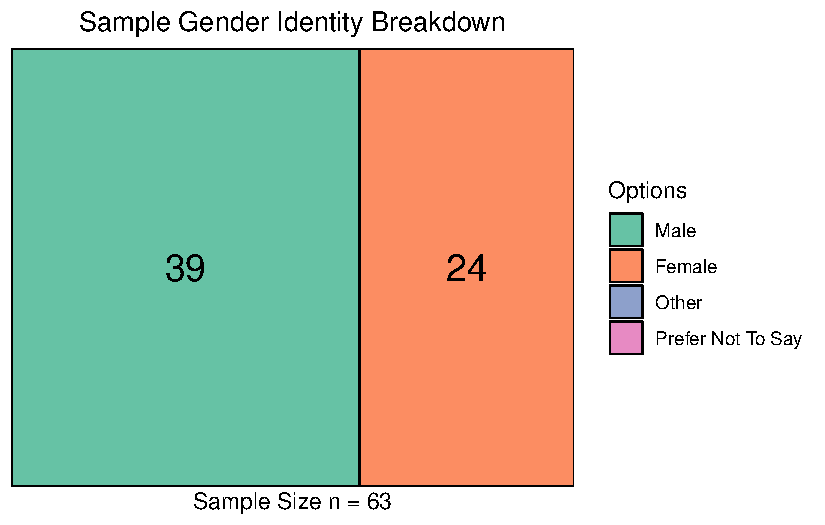
\includegraphics{technical_report_files/figure-pdf/p2-1.pdf}

Students picked up to 2 majors, with STA seeing a significant share of
responses.

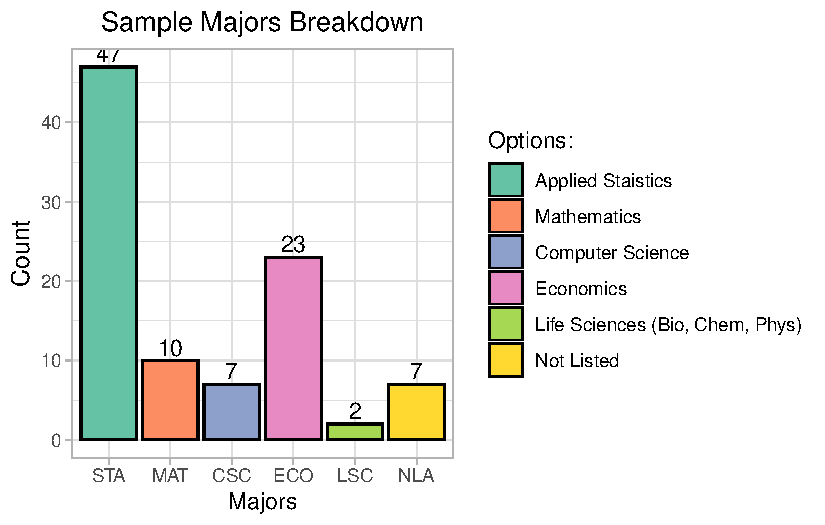
\includegraphics{technical_report_files/figure-pdf/p3-1.pdf}

We had almost an even balance of Domestic and International students in
our responses.

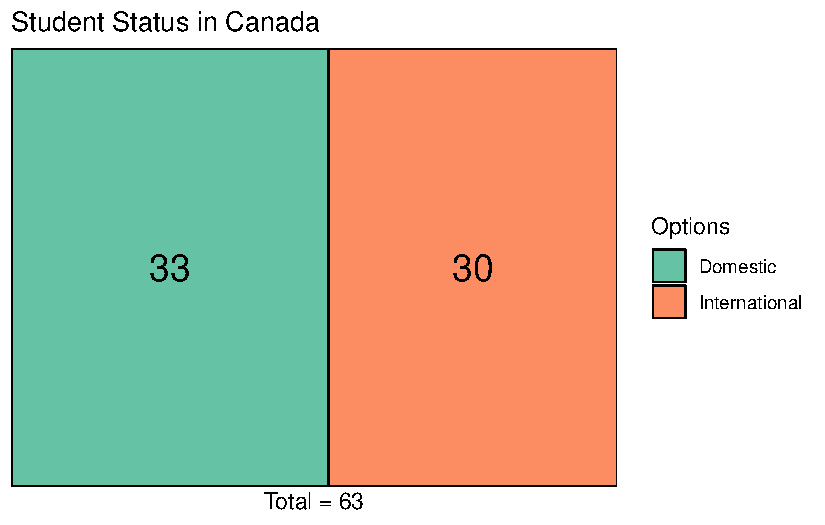
\includegraphics{technical_report_files/figure-pdf/p4-1.pdf}

Finally, we recorded students living distance from campus.

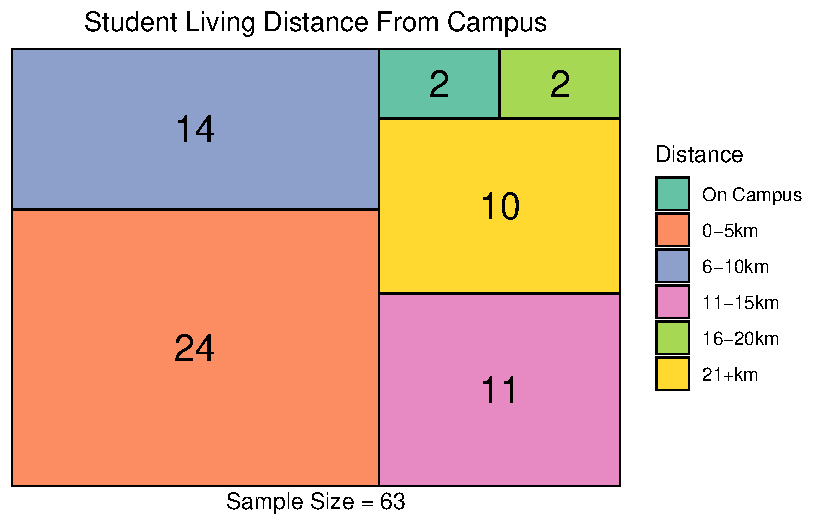
\includegraphics{technical_report_files/figure-pdf/p5-1.pdf}

\subsection{Research Question 1}\label{research-question-1}

In this question we aimed to explore and find out which is the most
preferred types of extracurricular activities whilst also examining
whether demographic factors such as major, demographics and student
status influence the preference for certain extracurricular activities.
By conducting this analysis we hope to gain an understanding of the
sample and the wider population in their extracurricular selection
habits.

\textbf{NOTE:} For easy analysis and ability to come up with clearer
conclusions, the Major column and the activity column were split into
different rows.

For the most preferred type of extracurricular activity, we were able to
get the count of students in the different extracurricular activities
and display a graph showing the counts of students in each
extracurricular activity.

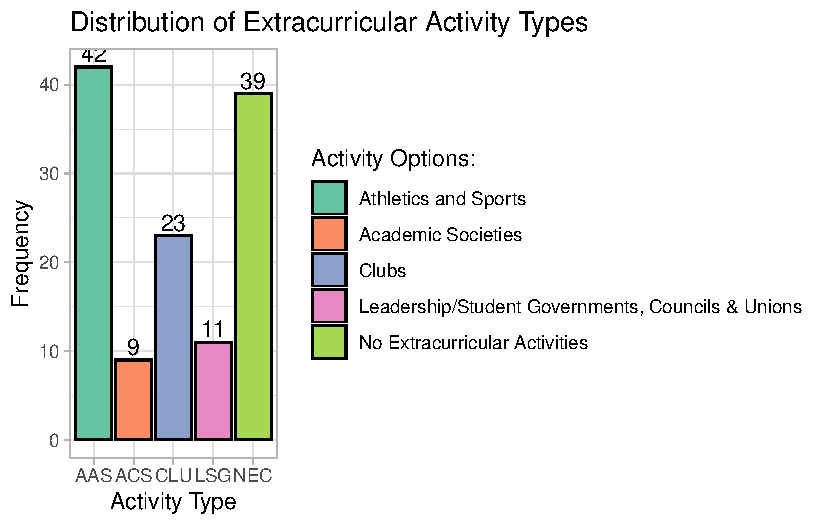
\includegraphics{technical_report_files/figure-pdf/rq1-1.pdf}

According to the bar plot, the most popular extracurricular activity
among students was Athletics and Sports (AAS) with and the least popular
extracurricular activity is Academic Societies (ACS) with students. It
was also particularly interesting to observe that most students do not
participate in Extracurricular Activities, making the NEC category
second in popularity.

To investigate the proportion of students participating in each activity
by demographic factors like Major, Student Status and Gender Identity,
we used two statistical tests, namely ANOVA and the T-Test.

Before we began with our tests we first conducted preliminary Assumption
Tests.

\subsubsection{Testing for the Significance of Majors on Activity
Proportion using the ANOVA
Test}\label{testing-for-the-significance-of-majors-on-activity-proportion-using-the-anova-test}

The Assumptions of ANOVA are:

\begin{enumerate}
\def\labelenumi{\arabic{enumi}.}
\tightlist
\item
  Normality: The data within each group should be normally distributed
\item
  Homogeneity of Variances: The variance of data within each group
  should be equal.
\item
  Random Sampling: Observations from each group have been sampled
  randomly and are independent of each other. (When we were collecting
  our sample this was already put into account)
\end{enumerate}

To test for Normality we used a Q-Q residuals plot.

\begin{verbatim}
             Df Sum Sq Mean Sq F value Pr(>F)
major         5   11.3   2.266   0.804  0.549
Residuals   118  332.5   2.818               
\end{verbatim}

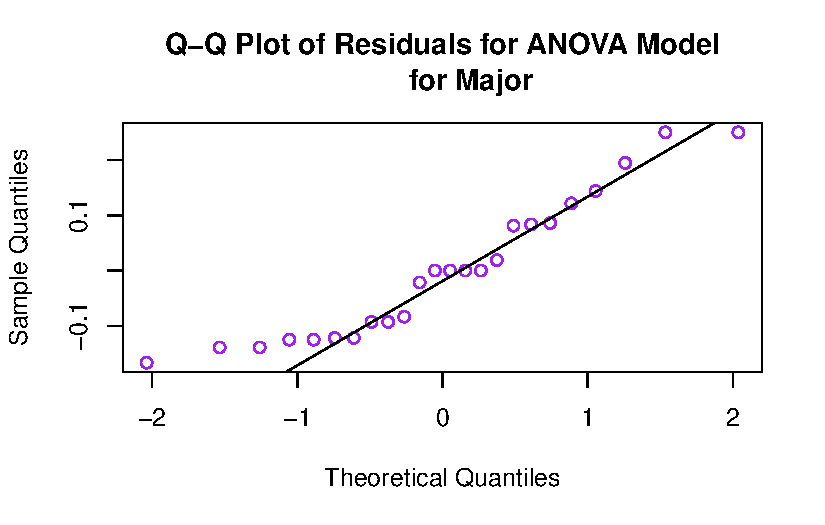
\includegraphics{technical_report_files/figure-pdf/r2-1.pdf}

From the plot we can observe that the points almost follow a straight a
line indicating that the residuals are normally distributed.

For the equality of variances within each group we used the Levene Test.

\textbf{\emph{Null Hypothesis}} (\(H_{o}\)) : The population variances
between the groups are equal.

\textbf{\emph{Alternative Hypothesis}} (\(H_{1}\)) : The population
variances between the groups are different.

\begin{longtable}[]{@{}lrrr@{}}
\caption{Levene Test}\tabularnewline
\toprule\noalign{}
& Df & F value & Pr(\textgreater F) \\
\midrule\noalign{}
\endfirsthead
\toprule\noalign{}
& Df & F value & Pr(\textgreater F) \\
\midrule\noalign{}
\endhead
\bottomrule\noalign{}
\endlastfoot
group & 5 & 0.3392478 & 0.8882135 \\
& 118 & NA & NA \\
\end{longtable}

We found our p value to be 0.8882135, which is greater than the
significance level value α = 0.05. This means we fail to reject the null
hypothesis and conclude that the assumption of equal variances is not
breached.

We then conducted the ANOVA Test to determine whether there are any
significant differences in the mean proportions of student Activity
Proportion and their respective majors.

\begin{longtable}[]{@{}lrrrrr@{}}
\caption{Anova}\tabularnewline
\toprule\noalign{}
& Df & Sum.Sq & Mean.Sq & F.value & Pr..F. \\
\midrule\noalign{}
\endfirsthead
\toprule\noalign{}
& Df & Sum.Sq & Mean.Sq & F.value & Pr..F. \\
\midrule\noalign{}
\endhead
\bottomrule\noalign{}
\endlastfoot
major & 5 & 11.3293 & 2.26586 & 0.8040241 & 0.5489808 \\
Residuals & 118 & 332.5417 & 2.81815 & NA & NA \\
\end{longtable}

From the ANOVA Analysis we can see that there is no statistical
significant difference in the proportion of extracurricular activity
participation across the different majors. The p- value of which is
greater than the significance level α = 0.05, concluded that we would
fail to reject the null hypothesis. The F-value of also shows us that
there is low variability between the group means.

The box plot below validates our results on that there is no significant
difference in activity participation across majors.

\subsubsection{Testing for the Significance of Gender on Activity
Proportion using the
T-Test}\label{testing-for-the-significance-of-gender-on-activity-proportion-using-the-t-test}

Before we begin with analysis, we must conduct preliminary tests to
ensure that we are fit to use this test.

Assumptions of the T-test are:

1. Random Variables: The observations must be independent.(When sampling
we took this into account)

2. Normality: The data in each group should be normally distributed.

3.Equality of Variances - The variances in the two groups should be
approximately equal. 4. The dependent variable should be measured on an
interval or ratio scale.(This has been met as our dependent variable is
the proportions of the people in each activity type) \textbf{\emph{Null
Hypothesis}} (\(H_{o}\)) : The population means between the groups are
equal.

\textbf{\emph{Alternative Hypothesis}} (\(H_{1}\)) : The population
means between the groups are different.

\begin{longtable}[]{@{}rr@{}}
\caption{Shapiro-Wilk Test}\tabularnewline
\toprule\noalign{}
W statistic & p-value \\
\midrule\noalign{}
\endfirsthead
\toprule\noalign{}
W statistic & p-value \\
\midrule\noalign{}
\endhead
\bottomrule\noalign{}
\endlastfoot
0.948502 & 0.6508111 \\
\end{longtable}

We conducted the Shapiro-Wilk Test to determine if the distribution in
both groups is normal. The p-value is 0.651 which is greater than the
significance level value of 0.05 indicating that the Genders are
normally distributed.

To test the second Assumption of equality of variances we used the
Levene Test.

\begin{longtable}[]{@{}lrrr@{}}
\caption{Levene Test}\tabularnewline
\toprule\noalign{}
& Df & F value & Pr(\textgreater F) \\
\midrule\noalign{}
\endfirsthead
\toprule\noalign{}
& Df & F value & Pr(\textgreater F) \\
\midrule\noalign{}
\endhead
\bottomrule\noalign{}
\endlastfoot
group & 1 & 1.817149 & 0.2145765 \\
& 8 & NA & NA \\
\end{longtable}

Our results confirmed that the variances are equal as the p-value was
0.2146 which is greater than 0.05 confirming the Homogeneity of
Variances property.

Now to conduct our analysis of the significance of Gender Identity on
activity proportion we opted to use both the t-test and the Wilcox Test
to validate our results as we had noted above that the normality was
violated hence why to have a confident answer we implemented both.

\begin{longtable}[]{@{}lrrrrr@{}}
\caption{T Test}\tabularnewline
\toprule\noalign{}
& T\_statistic & Df & p\_value & mean\_group1 & mean\_group2 \\
\midrule\noalign{}
\endfirsthead
\toprule\noalign{}
& T\_statistic & Df & p\_value & mean\_group1 & mean\_group2 \\
\midrule\noalign{}
\endhead
\bottomrule\noalign{}
\endlastfoot
t & 0 & 8 & 1 & 0.2 & 0.2 \\
\end{longtable}

\begin{longtable}[]{@{}lrr@{}}
\caption{Wilcox Test}\tabularnewline
\toprule\noalign{}
& W\_statistic & p\_value \\
\midrule\noalign{}
\endfirsthead
\toprule\noalign{}
& W\_statistic & p\_value \\
\midrule\noalign{}
\endhead
\bottomrule\noalign{}
\endlastfoot
W & 13 & 1 \\
\end{longtable}

From both the tests we can see that the p-value is 1 which is greater
than the significance level of 0.05 showing that there is no significant
difference between Females and Males in the Activity Participation
proportions. We therefore fail to reject the null hypothesis. We can
also see that both the genders have an average of 0.2.

Below, a box plot of the two genders has been plotted in order to
validate the results that indeed there is no significant difference
between Activity Type proportion and the gender.

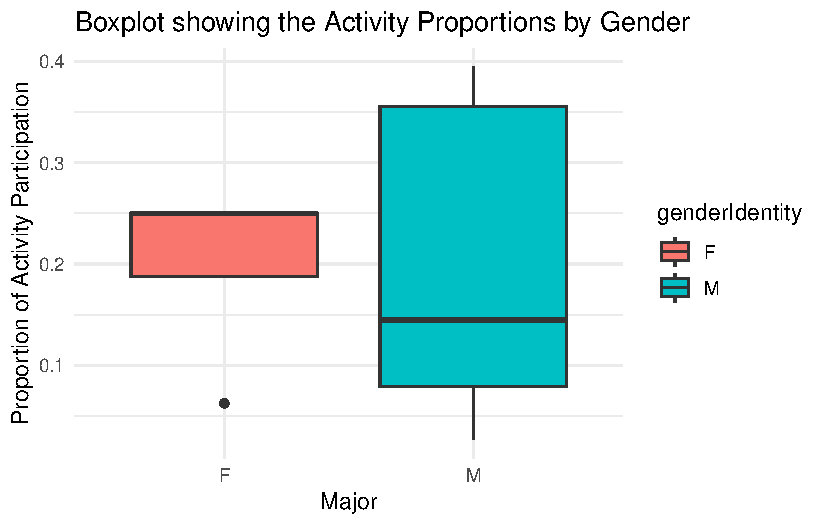
\includegraphics{technical_report_files/figure-pdf/r10-1.pdf}

\subsubsection{Testing for the Significance of Student Status on
Activity Proportion using the
T-Test}\label{testing-for-the-significance-of-student-status-on-activity-proportion-using-the-t-test}

We conducted preliminary tests before using the test and our results are
as shown below.

\begin{longtable}[]{@{}lr@{}}
\caption{Shapiro-Wilk Test}\tabularnewline
\toprule\noalign{}
studentStatus & shapiro\_p\_value \\
\midrule\noalign{}
\endfirsthead
\toprule\noalign{}
studentStatus & shapiro\_p\_value \\
\midrule\noalign{}
\endhead
\bottomrule\noalign{}
\endlastfoot
D & 0.7874026 \\
I & 0.7086627 \\
\end{longtable}

\begin{longtable}[]{@{}lrrr@{}}
\caption{Levene Test}\tabularnewline
\toprule\noalign{}
& Df & F value & Pr(\textgreater F) \\
\midrule\noalign{}
\endfirsthead
\toprule\noalign{}
& Df & F value & Pr(\textgreater F) \\
\midrule\noalign{}
\endhead
\bottomrule\noalign{}
\endlastfoot
group & 1 & 0.0022155 & 0.9636119 \\
& 8 & NA & NA \\
\end{longtable}

From our results of the Shapiro-Wilk test we can conclude that our
results are normal.This is because we can see that the p-value of
domestic students(0.787) and international students(0.709) are both
greater than 0.05 allowing us to reject the null hypothesis.

For the Homogeneity of Variances, due to the p value(0.9636) being
greater than 0.05 we can conclude that the variances of the both the
groups are relatively equal meaning that we fail to reject the null
hypothesis.

The results of our T-Test can be found below.

\begin{longtable}[]{@{}lrrrrr@{}}
\caption{T Test}\tabularnewline
\toprule\noalign{}
& T\_statistic & Df & p\_value & mean\_group1 & mean\_group2 \\
\midrule\noalign{}
\endfirsthead
\toprule\noalign{}
& T\_statistic & Df & p\_value & mean\_group1 & mean\_group2 \\
\midrule\noalign{}
\endhead
\bottomrule\noalign{}
\endlastfoot
t & 0 & 8 & 1 & 0.2 & 0.2 \\
\end{longtable}

From the test a p-value of 1 is greater than the significance level of
0.05 which indicates that there is no difference between Domestic and
International students in activity participation across the different
activity types therefore rejecting the null hypothesis.

Below is a Boxplot validating the results that we just proved,

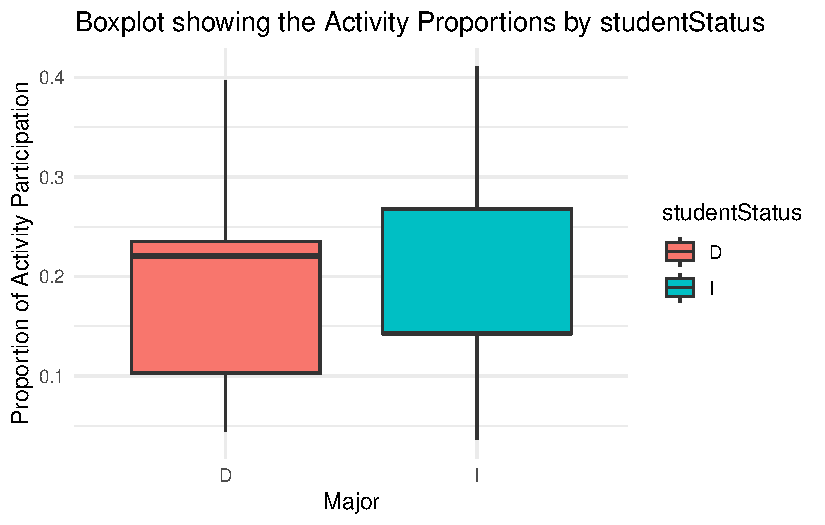
\includegraphics{technical_report_files/figure-pdf/r14-1.pdf}

\subsubsection{Conclusion on Research Question
1}\label{conclusion-on-research-question-1}

We can therefore conclude that indeed demographic factors have no
significant effect on the preference for certain extracurricular
activities. We also noted that the most popular type of extracurricular
activity amongst students was Athletics and Sports(AAS).

\subsection{Research Question 2}\label{research-question-2}

In RQ2, we analysed if the proximity to campus affects one's ability to
participate in extracurricular activities.

\begin{itemize}
\tightlist
\item
  Null Hypothesis (\(H_{o}\)): Proximity to campus (campusDistance) does
  not affect participation in extracurricular activities.
\item
  Alternative Hypothesis (\(H_{1}\)): Proximity to campus
  (campusDistance) has an effect on participation in extracurricular
  activities.
\end{itemize}

\subsubsection{Campus Distance and Activity
Count}\label{campus-distance-and-activity-count}

Statistical Test: To evaluate this, we used the correlation analysis
test between campus distance and the number of extracurricular
activities using Pearson's correlation test. Prior to conducting this
test, we will verify the assumptions for the test first.

\begin{longtable}[]{@{}lrr@{}}
\caption{Correlation Analysis}\tabularnewline
\toprule\noalign{}
Statistic & CampusDistance & ActivityCount \\
\midrule\noalign{}
\endfirsthead
\toprule\noalign{}
Statistic & CampusDistance & ActivityCount \\
\midrule\noalign{}
\endhead
\bottomrule\noalign{}
\endlastfoot
Min & 0.000000 & 0.000000 \\
1st Quartile & 1.000000 & 0.000000 \\
Median & 2.000000 & 1.000000 \\
Mean & 2.193548 & 1.451613 \\
3rd Quartile & 3.000000 & 2.000000 \\
Max & 5.000000 & 4.000000 \\
\end{longtable}

The descriptive statistics suggest that most students live fairly close
to campus (within 2-3 units) and participate in 1-2 extracurricular
activities. This variability in both campusDistance and activityCount
supports further analysis to see if there's a relationship between
proximity and participation.

\begin{figure}

\centering{

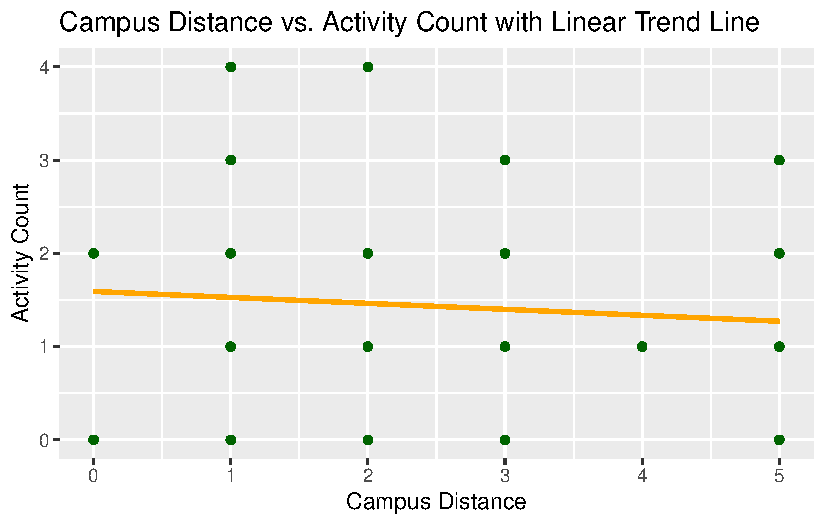
\includegraphics{technical_report_files/figure-pdf/fig-plot1-1.pdf}

}

\caption{\label{fig-plot1}Scatter Plot}

\end{figure}%

Moving on we inspect the relationship between the variables. As it can
be seen from Figure~\ref{fig-plot1}, there seems to be no linear
relation between the variables.

\begin{figure}[H]

{\centering 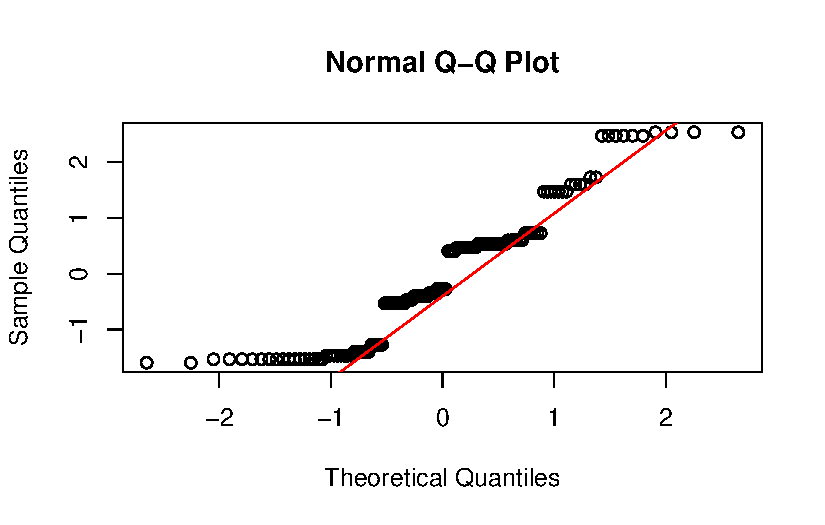
\includegraphics{technical_report_files/figure-pdf/plot2-1.pdf}

}

\caption{Scatter Plot}

\end{figure}%

The Q-Q plot displays how the residuals (differences between observed
and fitted values) align with the normal distribution. In this case,
residuals do not fully align along the red diagonal line, indicating
that normality is somewhat violated. The observed points deviate in a
stepwise manner, particularly at the tails, which suggests potential
non-normality in residuals.

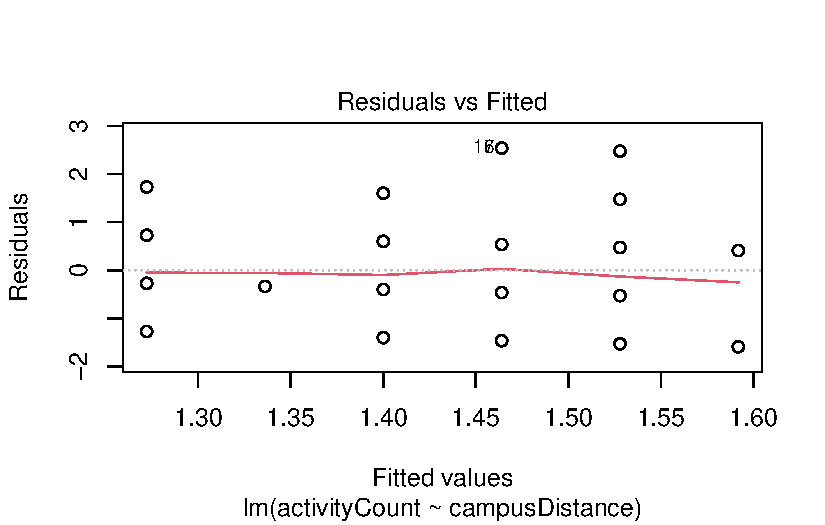
\includegraphics{technical_report_files/figure-pdf/plot3-1.pdf}

This plot helps in identifying any non-linearity, unequal variance
(heteroscedasticity), or outliers. Here, residuals seem randomly
scattered around the fitted line with no obvious pattern, suggesting
homoscedasticity (constant variance). However, a few points like 33, 9,
and 15 appear as potential outliers, which might influence the results.

Since there is non-normality between these variables, we proceed with
Spearman's rank correlation to analyze the association between campus
distance and activity count.

\begin{longtable}[]{@{}
  >{\raggedright\arraybackslash}p{(\columnwidth - 6\tabcolsep) * \real{0.3239}}
  >{\raggedleft\arraybackslash}p{(\columnwidth - 6\tabcolsep) * \real{0.3380}}
  >{\raggedleft\arraybackslash}p{(\columnwidth - 6\tabcolsep) * \real{0.1127}}
  >{\raggedright\arraybackslash}p{(\columnwidth - 6\tabcolsep) * \real{0.2254}}@{}}

\caption{\label{tbl-plot4}Correlation Test Results}

\tabularnewline

\caption{Summary of Correlation Test Results}\tabularnewline
\toprule\noalign{}
\begin{minipage}[b]{\linewidth}\raggedright
Test
\end{minipage} & \begin{minipage}[b]{\linewidth}\raggedleft
Correlation\_Coefficient
\end{minipage} & \begin{minipage}[b]{\linewidth}\raggedleft
p\_value
\end{minipage} & \begin{minipage}[b]{\linewidth}\raggedright
Significance
\end{minipage} \\
\midrule\noalign{}
\endfirsthead
\toprule\noalign{}
\begin{minipage}[b]{\linewidth}\raggedright
Test
\end{minipage} & \begin{minipage}[b]{\linewidth}\raggedleft
Correlation\_Coefficient
\end{minipage} & \begin{minipage}[b]{\linewidth}\raggedleft
p\_value
\end{minipage} & \begin{minipage}[b]{\linewidth}\raggedright
Significance
\end{minipage} \\
\midrule\noalign{}
\endhead
\bottomrule\noalign{}
\endlastfoot
Pearson's Correlation & -0.018 & 0.891 & Not Significant \\
Spearman's Correlation & 0.025 & 0.847 & Not Significant \\

\end{longtable}

The Spearman's rank correlation test results are as follows:

\begin{itemize}
\tightlist
\item
  Spearman correlation coefficient: 0.025
\item
  p-value: 0.847
\end{itemize}

This result indicates a very weak positive correlation between
\texttt{campusDistance} and \texttt{activityCount}, but it is not
statistically significant (p-value \textgreater{} 0.05). Therefore, we
fail to reject the null hypothesis, suggesting no significant
association between proximity to campus and participation in
extracurricular activities based on this data.

\subsection{Research Question 3}\label{research-question-3}

In RQ3, we analyzed if the the timing, the time spent on extra
curricular activity affected one's level of participation in
extracurricular activities.

\begin{itemize}
\tightlist
\item
  Null Hypothesis (\(H_{o}\)): Time Commitment (timeCommitment) does not
  affect participation levels in extracurricular activities.
\item
  Alternative Hypothesis (\(H_{1}\)): Time Commitment (timeCommitment)
  has an effect on participation levels in extracurricular activities.
\end{itemize}

We used the variables of student involvement (studentInvolvement) and
activity count (activityCount) to represent the participation levels.

\subsubsection{Time Commitment and Student
Involvement}\label{time-commitment-and-student-involvement}

\textbf{Statistical Test}: To evaluate this, we used the correlation
analysis test between time commitment and student involvement variables
using Spearman's correlation test. Before proceeding with the test, we
will verify the assumptions for the test.

\textbf{Normality of Variables}: In our exploration we found that the
variables of timeCommitment (TC), and studentInvolvement (SI) are not
normally distributed as seen by the QQ plots in
Figure~\ref{fig-normality-of-variables} as they deviate from the
normality line. Hence we proceeded to apply the correlation test using
the Spearman's rank coefficient instead of Pearson's coefficient
(requiring normality).

\begin{figure}

\centering{

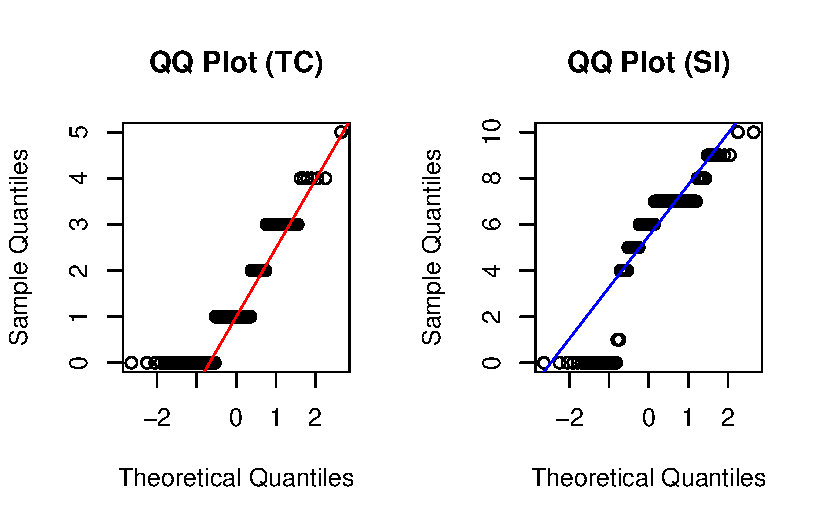
\includegraphics{technical_report_files/figure-pdf/fig-normality-of-variables-1.pdf}

}

\caption{\label{fig-normality-of-variables}Normality of Variables}

\end{figure}%

\textbf{Monotonic Association}: Next we confirmed the assumption of
Spearman's rank coefficient test requiring a monotonic relationship
between the variables (timeCommitment and studentInvovlement). We found
that the relationship between these variables was monotonic,
specifically increasing as seen in
Figure~\ref{fig-scatter-plot-involvement}.

\begin{figure}

\centering{

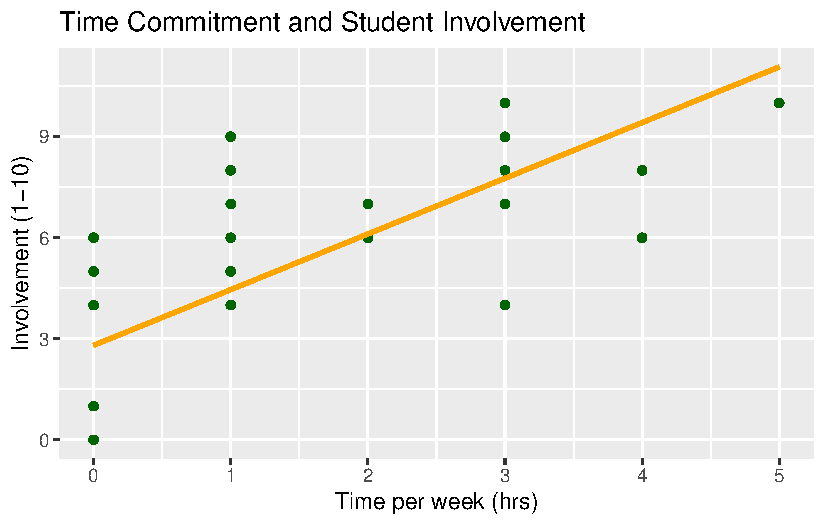
\includegraphics{technical_report_files/figure-pdf/fig-scatter-plot-involvement-1.pdf}

}

\caption{\label{fig-scatter-plot-involvement}Checking Monotonicity}

\end{figure}%

\textbf{Results}: As seen in Table~\ref{tbl-spear-corr}, the Spearman's
rank correlation coefficient is 0.808, which indicates a strong positive
correlation, pointing to a significant monotonic relationship between
timeCommitment and studentInvolvement. p-value is \textless{} 0.05,
hence the correlation is statistically significant, and we can reject
the null-hypothesis.

\begin{longtable}[]{@{}ll@{}}

\caption{\label{tbl-spear-corr}Correlation Test Results}

\tabularnewline

\caption{Spearman's Rank Correlation Results}\tabularnewline
\toprule\noalign{}
Statistic & Value \\
\midrule\noalign{}
\endfirsthead
\toprule\noalign{}
Statistic & Value \\
\midrule\noalign{}
\endhead
\bottomrule\noalign{}
\endlastfoot
Spearman Coefficient (rho) & 0.744 \\
p-value & 4.608e-23 \\

\end{longtable}

Hence students who spend more time in the activities have higher
participation in extra curricular activities measured by the activity
count, as suggested by the strong association based on our data.

\subsubsection{Time Commitment and Activity
Count}\label{time-commitment-and-activity-count}

We wanted to check whether the time commitment and participation
measured by the activityCount variable were correlated.

\textbf{Statistical Test}:

As discussed before, both the timeCommitment and activityCount variables
did not meet normality assumptions, so we proceed with the Spearman's
rank correlation coefficient as our statistical test.

\textbf{Normality of Variables}:

To proceed with this test, we used QQ-plots to verify normality of
timeCommitment (TC) and activityCount(AC). As seen in
Figure~\ref{fig-normality-activity} they are non-normal variables due to
their deviation from the normal line.

\begin{figure}

\centering{

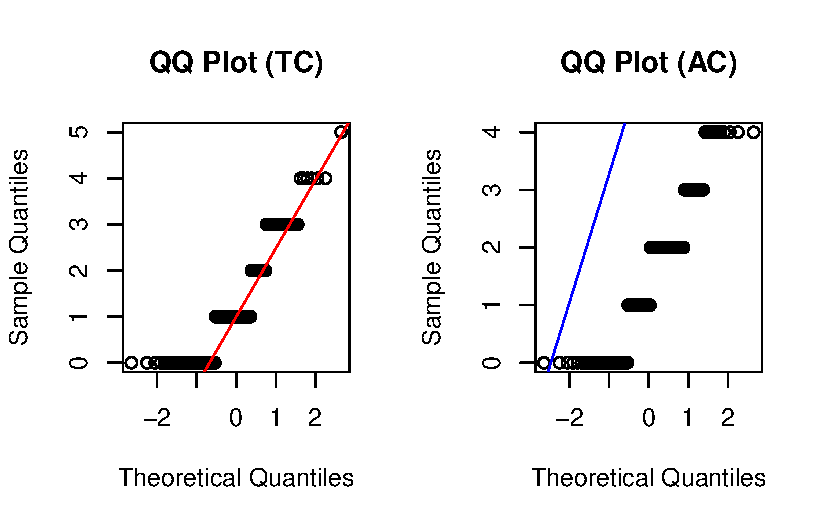
\includegraphics{technical_report_files/figure-pdf/fig-normality-activity-1.pdf}

}

\caption{\label{fig-normality-activity}Normality of Variables}

\end{figure}%

\textbf{Monotonic Association}: We confirmed that the relationship
between these variables was monotonic, specifically increasing as seen
in Figure~\ref{fig-monotonic-activity}

\begin{figure}

\centering{

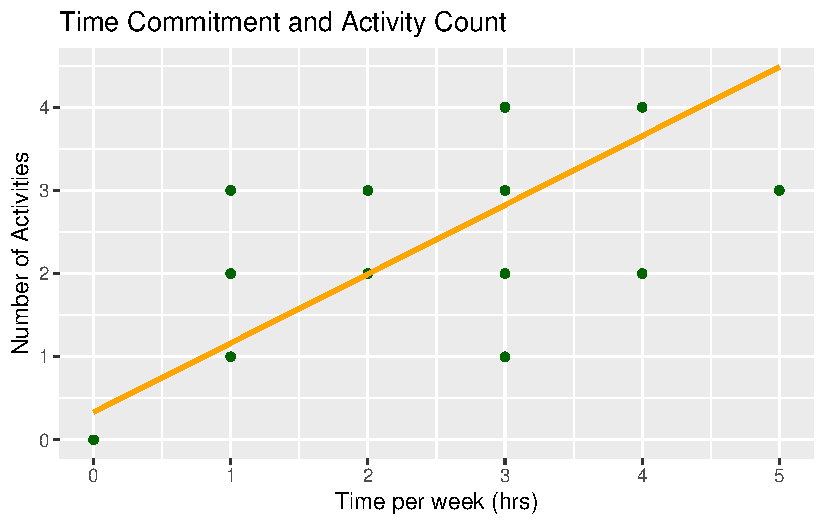
\includegraphics{technical_report_files/figure-pdf/fig-monotonic-activity-1.pdf}

}

\caption{\label{fig-monotonic-activity}Checking Monotonicity}

\end{figure}%

\begin{longtable}[]{@{}ll@{}}
\caption{Correlation Test Results}\tabularnewline
\toprule\noalign{}
Statistic & Value \\
\midrule\noalign{}
\endfirsthead
\toprule\noalign{}
Statistic & Value \\
\midrule\noalign{}
\endhead
\bottomrule\noalign{}
\endlastfoot
Spearman Coefficient (rho) & 0.886 \\
p-value & 1.227e-42 \\
\end{longtable}

\textbf{Results}: The test results show that the coefficient value is
0.937, indicating a strong positive relationship. This would mean as
time commitment increases, so does activity count. The p-value is
\textless{} 0.05 and indicates strong evidence against the null
hypothesis, hence the relationship is unlikely due to chance.

Hence, these results indicate a strong, statistically significant
monotonic relationship between time commitment and activity count. As
students increase their time commitment, so does their participation
measured by involvement.

\section{Limitations}\label{sec-data3}

This study aimed to understand the reasons why students select and
participate in ECAs at UTM. Although our results did not yield
significant findings, several limitations may have contributed to this
outcome: One such notable limitation is the way in which our data was
collected. Although we proposed Stratified Random Sampling to collect
our data, we ended up collecting with Simple Random Sampling. This
likely lead to higher variance in our analysis and as a result, weaker
conclusions. Another big limitation is the possibility of non-response
bias in our sampling. Although the survey was distributed in a way that
made it available to all students, in effect if certain students we're
choosing not to respond to surveys, their chance of being selected would
be zero. In future studies, a better sampling methodology would have
been to use StRS with either SRS or Systematic Sampling within the
strata. If the study were to be repeated, there would be a number of
changes we would like to make in addition to modifying the sampling
methodology. We would change the student major question from multiselect
to a select one and instruct students to select the major they commit
the most time to; this would allow us to streamline and simplify the
analysis. The question regarding days of the week could likely be
dropped as it proved unbeneficial. This question could be instead
replaced with one regarding what time of day students spend most in
ECAs. Finally, we would likely change the question regarding students
living distance from campus to commute distance. Since the study is
interested in what factors affect ECA participation, considering commute
distance would be more likely to provide useful information, as two
students living the same distance from campus could have vastly
different commute times and thus have different amounts of time they can
spend on ECAs.

\section{Conclusion}\label{conclusion}

This study aims to explore this by investigating the reasons that
students select certain extracurricular activities at the University of
Toronto Mississauga campus (UTM). Analysis on the preferred types of
extracurricular activities whilst also examining whether demographic
factors influence these preferences showed that although the most
popular type of ECAs amongst students was Athletics and Sports,
demographic factors such as gender, student status and program of study.
Regarding, the proximity to campus and one's ability to participate in
ECAs, there indicated a very weak positive relationship between the
distance from campus and the number of activities that students engage
in. Unfortunately, this relationship is not statistically significant.
Finally, analysis on the time spent on ECAs indicates that there is a
strong statistically significant relationship between time commitment
and activity count. Notably, in the future, it would be more beneficial
to consider time commuting as a variable of interest than distance from
campus. Additionally, modifying the sampling methodology would be an
important change if this study were to be repeated by other researchers.

\newpage

\section{References}\label{references}



\end{document}
